\documentclass[8pt, twocolumn]{article}
\usepackage{stfloats}
\usepackage[utf8]{inputenc}
\usepackage{graphicx}
\usepackage[font=small]{caption}

% Set the margins
\usepackage[a4paper, total={6in, 8in}]{geometry}


\newcommand\wordcount{
   \immediate\write18{wordcount.bat \jobname.tex}
   \input{\jobname.wc}
}

\begin{document}

% Title Page
\begin{titlepage}
  \centering
  \vspace*{60px}
  \huge{Protein-Lithography Enhanced Digital Microfluidics} \\
  \Large{Bioactivation of Feedback Glass} \\
  \vspace{10px}
  \begin{tabular}{rl}
      \large{\textbf{Student:}} & \large{Francisco Javier Quero} \\
      \large{\textbf{Principal Investigator:}} & \large{Clemens Kaminski} \\
      \large{\textbf{Industrial Supervisor:}} & \large{Urs Gaudenz} \\
      \large{\textbf{Dayly Supervisor:}} & \large{Francesca van Tartwijk} \\
  \end{tabular}
  \vfill
  \today
  \vfill
\end{titlepage}


% Abstract
\clearpage
\onecolumn

\begin{abstract}
  \vspace{10px}

  In this project, we aim to bridge one of the most significant gaps between digital microfluidics technology, specifically electrowetting-on-dielectric, and its key application in the development of lab-on-a-chip devices. Despite considerable technological advancements in the past decade, including more robust chips, increased numbers of electrodes, and the integration of certain levels of actuators within chips, a disconnection still exists between the biochemical layer of the droplets driven inside and the devices' hardware.
  
  % \vspace{10px}
  
  We will work to bioactivate the surfaces within OpenDrop chips, one of the most widespread open-source platforms in the field, by binding proteins to the Tin-Indium-Oxide crystal covering the reactions, aiming to make it reactive to the chemical composition of the droplets driven inside the platform. Our focus will be on characterizing each step to identify the most optimal processes and troubleshoot potential issues. Ultimately, we will explore the interaction of these bioactivated surfaces with the machine's electronic feedback circuit, investigating whether this bioactivation could potentially detect different chemical processes occurring within the droplets.
  
  \end{abstract}

\clearpage
\twocolumn

% Main Body
\newpage
\section*{Introduction}

\begin{figure}[!b]
  \centering
  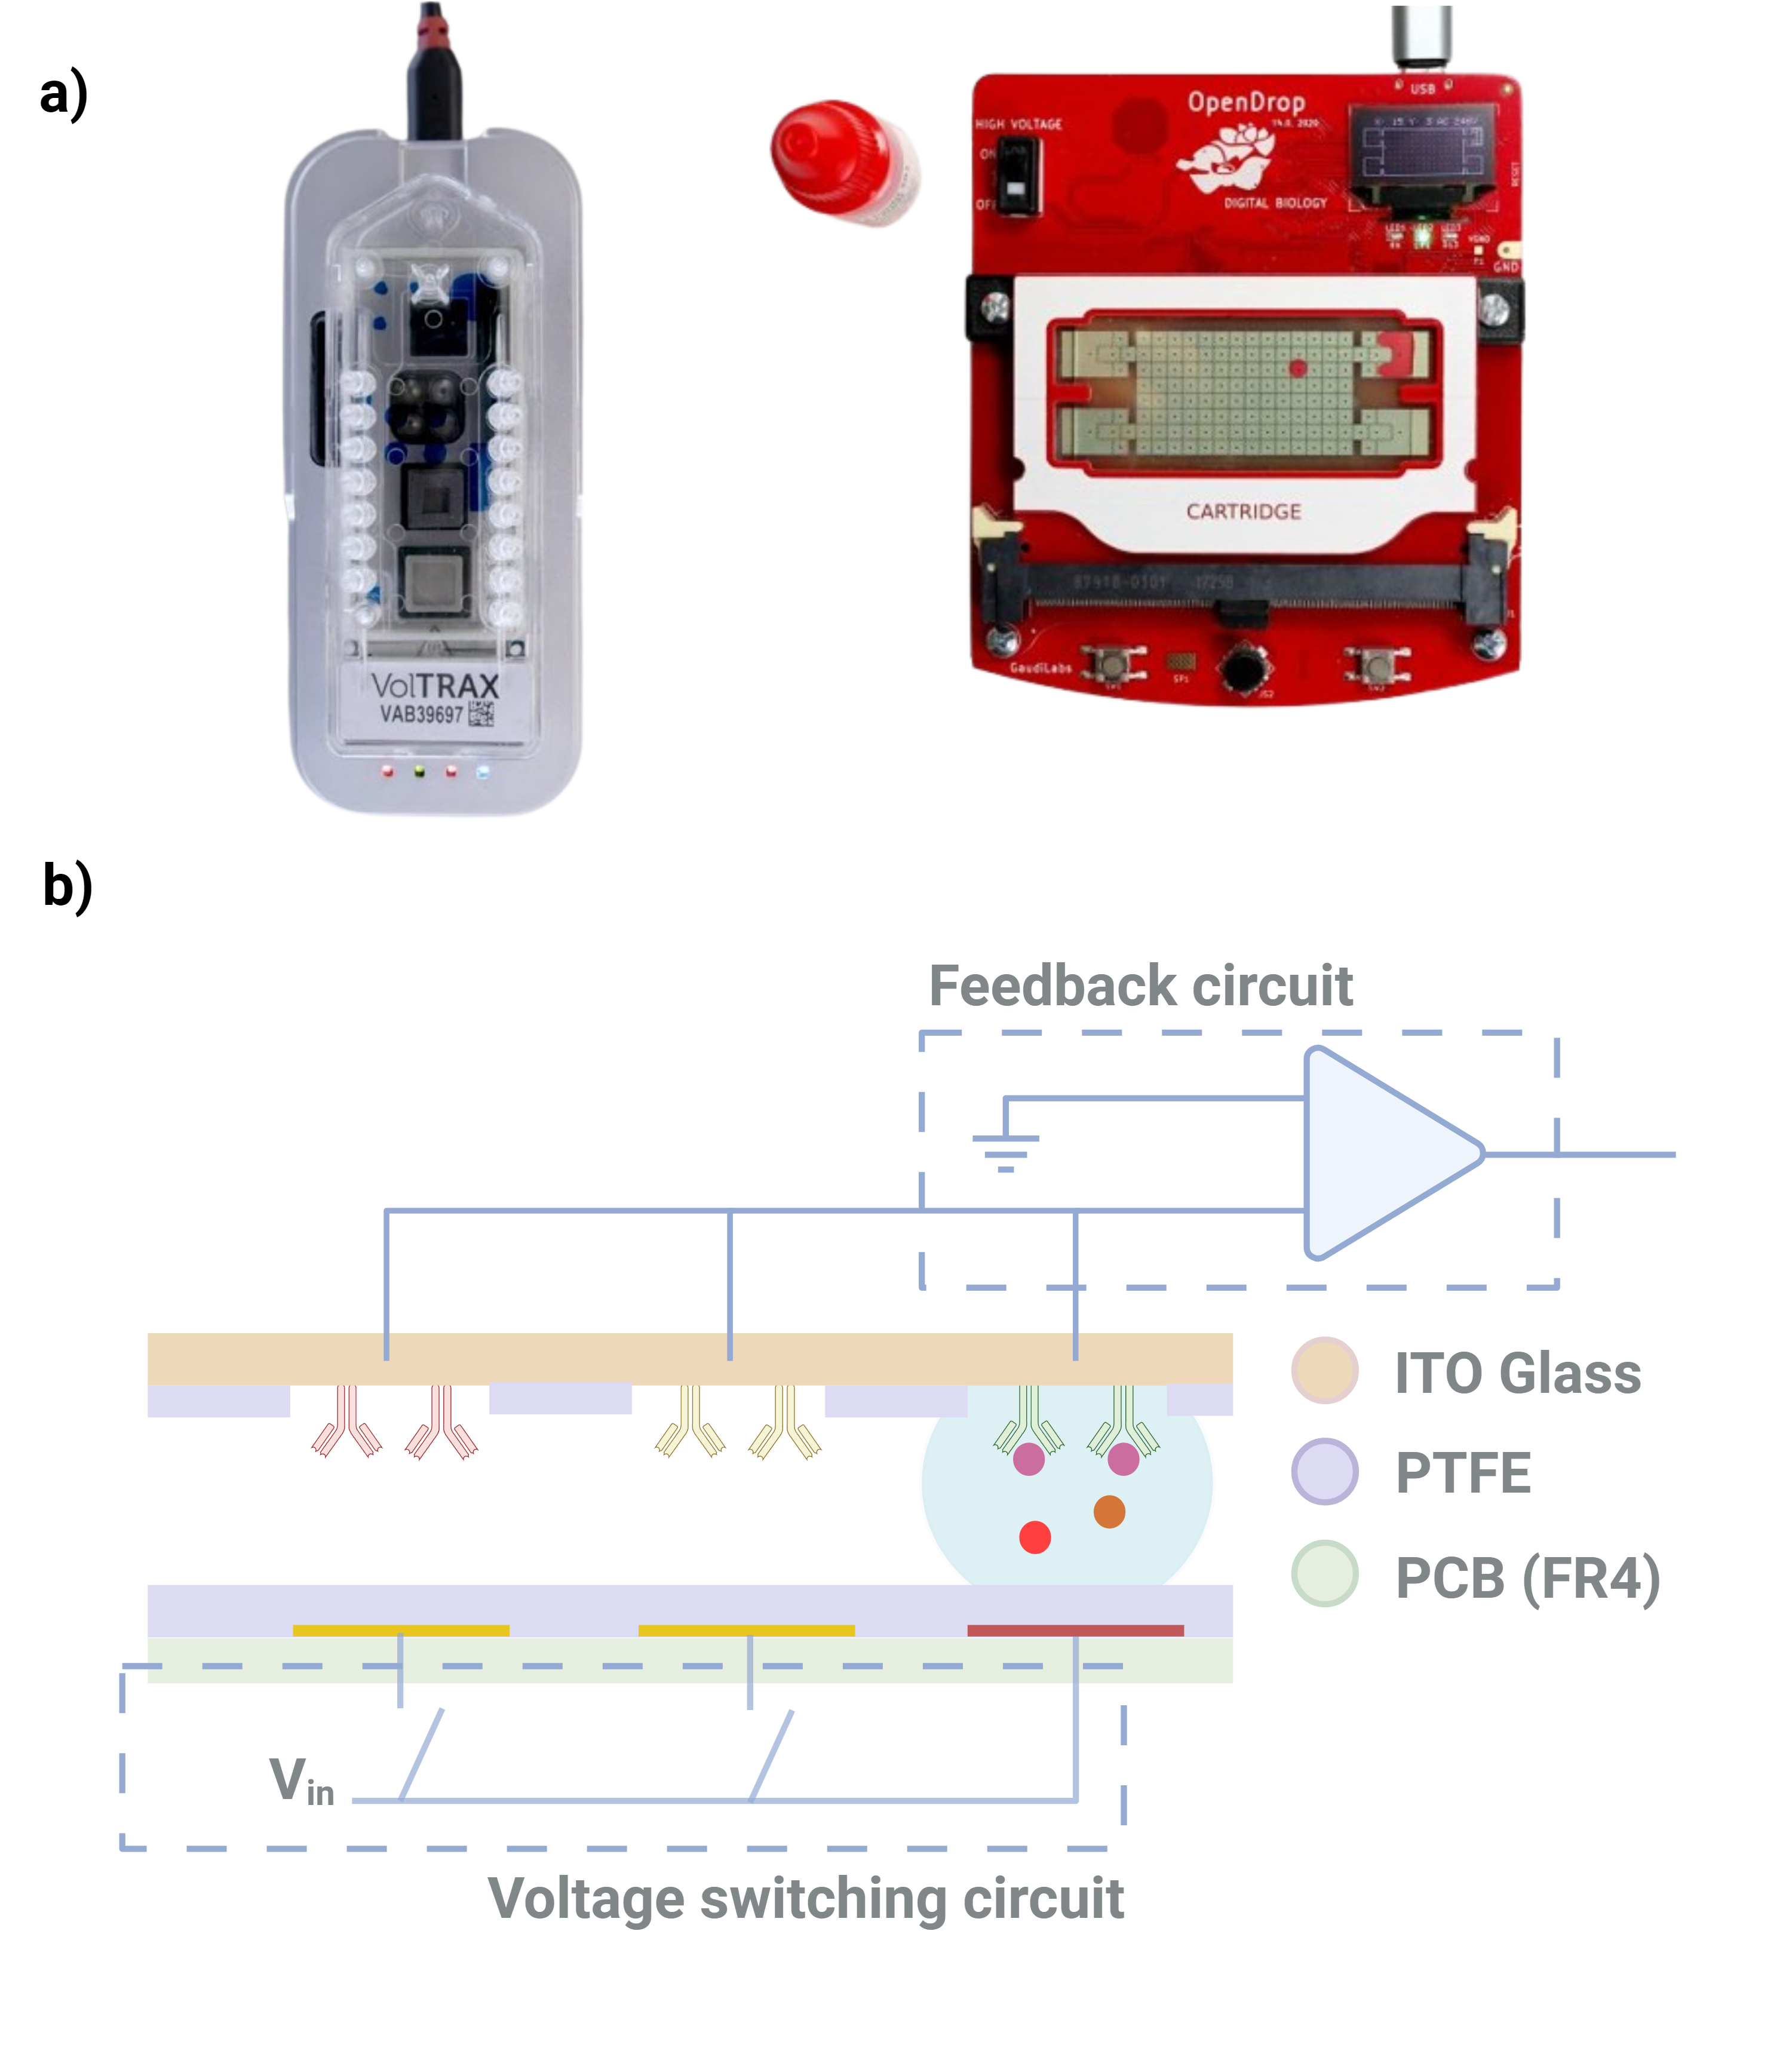
\includegraphics[width=\linewidth]{img/1.png}
  \caption{(a) Two of the most relevant digital microfluidics platforms: VolTRAX from Oxford Nanopore (left) and OpenDrop v4 from Gaudilabs (right). (b) Schematic of the working principle of digital microfluidics, with representation of the layers involved.}
  \label{fig:diagram}
\end{figure}

Digital microfluidics (DMF) is a field dedicated to automating laboratory procedures by harnessing a variety of technologies to facilitate an interface between programmable digital software and the controlled movement of fluids at the microfluidic scale.  In this project, we will specifically focus on a branch of DMF known as electrowetting-on-dielectric (EWOD) which utilizes the positioning of electrical charges beneath a thin, highly hydrophobic insulating layer to locally reduce the repulsion forces between the layer and the polar fluid droplets, thus facilitating their controlled movement \cite{beniContinuousElectrowettingEffect1982}. In the past ten years, substantial investments have been made in the field by both public organizations and private corporations \cite{liCurrentCommercializationStatus2020} allowing for swift technological progress in both the simplification and cost-reduction of hardware \cite{zhang2DLargescaleEWOD2020}, as well as greater miniaturization and an increase on electrode numbers \cite{qinSolutionMassProduction2021}. Currently, the principal challenge for EWOD is the integration of sensors into the chips, particularly chemical and biosensors, since most relevant sensing technologies are dependent on external costly and bulky optical detection systems \cite{huAllinOneDigitalMicrofluidics2022}.

To achieve this, we plan to bioactivate the crystal covering the electrodes, under which the microdroplets moves, leveraging on an existing protein patterning method \cite{straleMultiproteinPrintingLightInduced2016}. This will enable specific molecular interactions between the surface of the electrowetting device and the molecules inside the microdroplets. However, a significant challenge is the Polytetrafluoroethylene (PTFE) layer, a hydrophobic material coating the crystal, which aids droplet movement but hinders protein binding to the crystal surface (Figure \ref{fig:diagram}). During this project, we will work to develop a simple process for creating patterns that locally remove the hydrophobic layer, thereby exposing areas of the crystal for protein binding and subsequent interaction with the droplets. Finally, we plan to investigate how this binding mechanism affects the droplet positioning feedback system of the platform, particularly in measuring changes in capacitance related to the biomolecules on the glass alone and in their bound state with the droplet molecules \cite{wangUltraSensitiveCapacitiveMicrowire2019}.

The practical benefits of a platform capable of biologically interacting with the microdroplets are several. Whether as an \textit{actuator}, selectively binding (and quelating) proteins, cells, or other compounds from a solution, or as a \textit{sensor}, measuring real-time factors such as cell types proportions, DNA/RNA elements, or molecular concentrations in cell-containing or cell-free mixtures. In this way, we aim to bring EWOD-based digital microfluidics beyond mere fluid movement automation, becoming a comprehensive platform that measures and interacts with the biochemical layer of the microdroplets driven inside.

\newpage
\subsection*{The Platform: OpenDrop v4}

Traditionally, digital microfluidics has been reliant either on do-it-yourself (DIY) systems, crafted in-house within laboratories, or on highly expensive systems, designed for very specific experimental work in well-funded and equipped labs. OpenDrop v4 \ref{fig:cartridge} addresses this issue by utilizing standard Printed Circuit Board (PCB) manufacturing methods, which are easily scalable, and open-source hardware, which facilitates the customization of specific hardware components. As a result, OpenDrop emerges as a platform that is not only simple and cost-effective to replicate and adapt but also offers precision levels comparable to other platforms mentioned in the scientific literature \cite{alistarOpenDropIntegratedDoItYourself2017}.

Moreover, the fourth version of OpenDrop introduces a modular system based on `cartridges' \cite{OpenDropV4OpenDrop2020}. Researchers using this platform are not required to design the entire device; instead, they only need to develop the cartridge, which includes the electrode pattern and all the sensors surrounding them. These cartridges connect to the main board through standard connectors, allowing for easy system operation \ref{fig:cartridge}. This modularity is crucial as it enables us to design our own cartridges without the need to reinvent the core control system.

\begin{figure}[h]
  \centering
  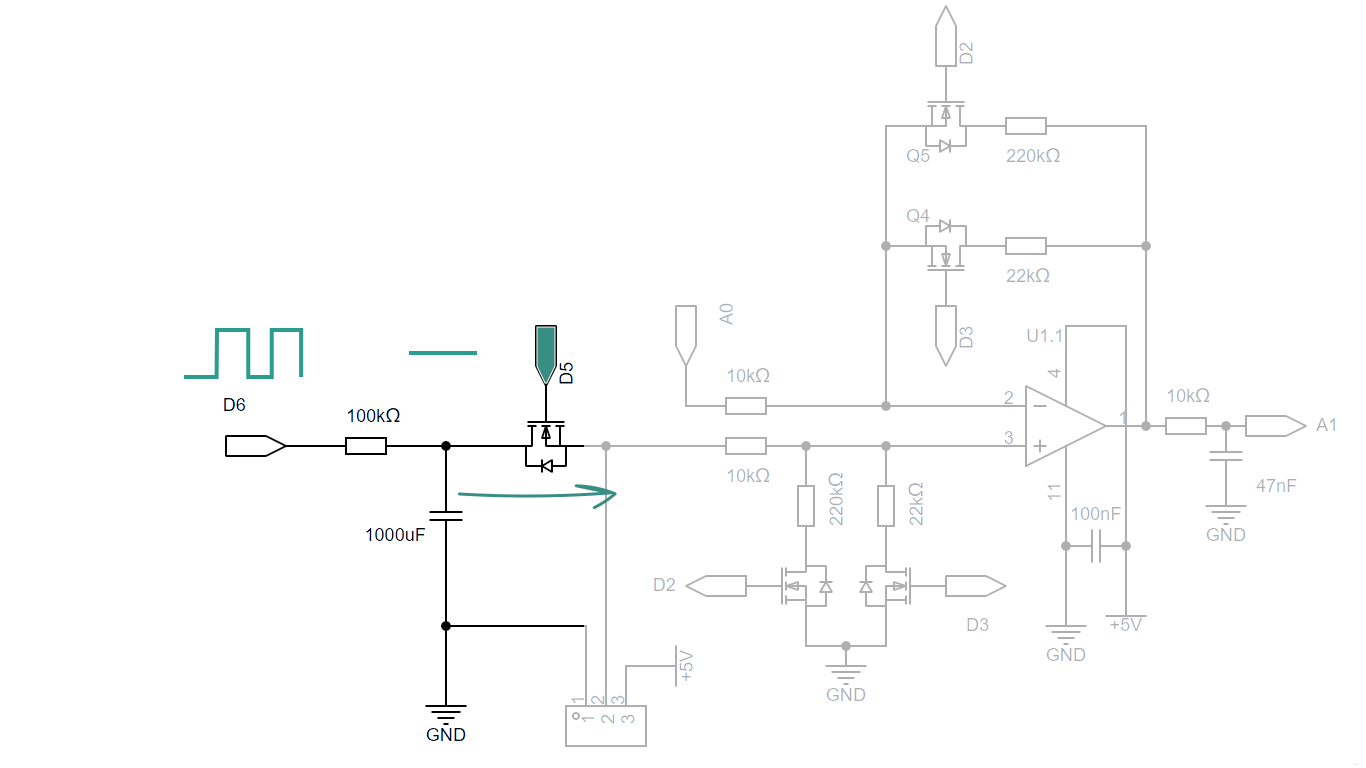
\includegraphics[width=\linewidth]{img/2.png}
  \caption{Representation of the OpenDrop v4 with plugged-in modular cartridge (top) and exploded diagram of the different cartridge layers (bottom). The microdroplets hover above the hydrophobic layer and below the ITO glass, which is also coated beneath with a layer of hydrophobic material (PTFE). Images obtained from \cite{OpenDropV4OpenDrop2020}.}
  \label{fig:cartridge}
\end{figure}

\subsection*{Patterning Proteins}

A primary challenge in our approach lies on the structure of the Indium Tin Oxide (ITO) glass, the layer to which proteins must be bound. This glass rquires an hydrophobic covering, allowing the electrodes to decrease this hydrophobicity locally by applying a voltage underneath, thereby driving the droplets to the less hydrophobic areas. On the other hand, since proteins bind to the glass underneath the fluoropolymer, they must be exposed to the fluid so it becomes necessary to locally remove the hydrophobic layer, allowing proteins and droplets to be contact. The key is that the hydrophobic removal must be subtle enough so that the interaction between the droplet and the crystal does not overshadow the potential repulsion of the hydrophobic layer when the electrode is turned off.

\subsubsection*{Exposing the ITO Glass Over the Hydrophobic Cover Layer}


\begin{figure}[!b]
  \centering
  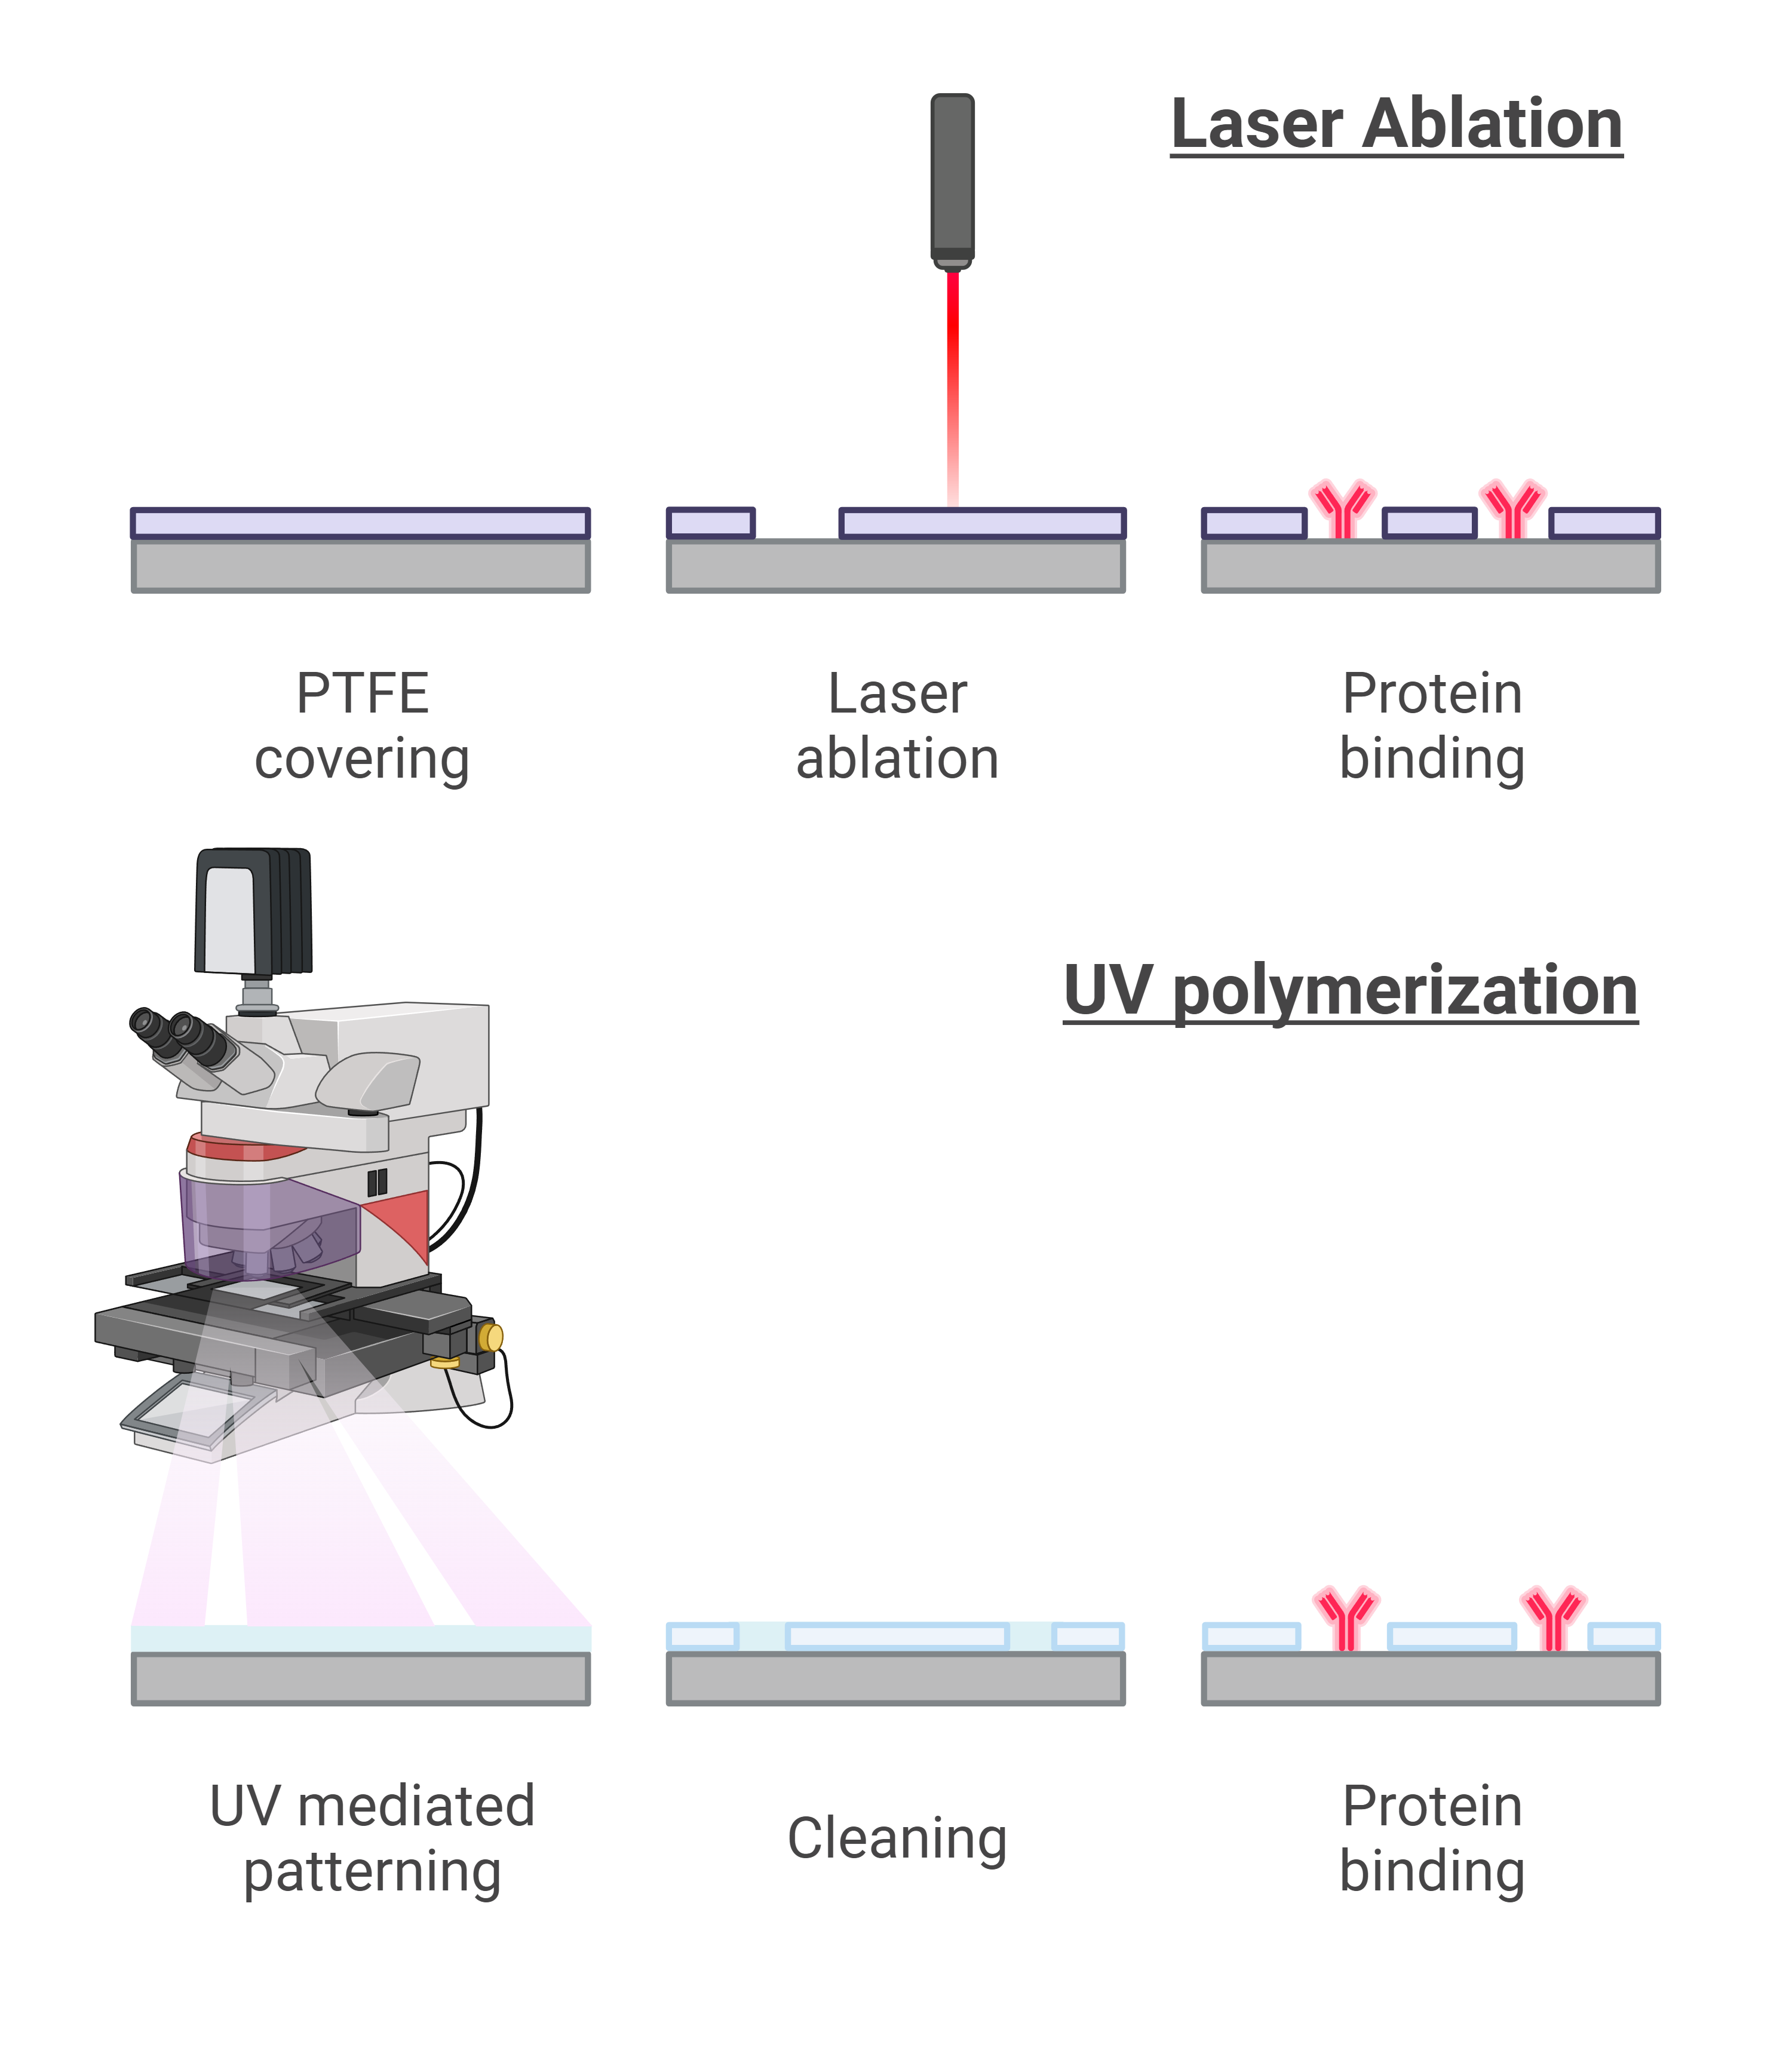
\includegraphics[width=\linewidth]{img/3.png}
  \caption{Representation of the two methods proposed to pattern the hydrophobic layer, laser ablation (top) and UV polymerisation (bottom).}
  \label{fig:methods}
\end{figure}

There are two potential methods to expose the ITO glass beneath the hydrophobic layer:

\begin{enumerate}
    \item \textbf{Laser Ablation}: The entire glass surface can be covered with a standard fluoropolymer, as per OpenDrop manufacturing manuals, followed by using a laser to ablate the areas of interest \cite{rodriguez-alabandaStudyMainInfluencing2019}. This approach initially seems simpler, utilizing readily available equipment such as a laser cutter from the maker lab. However, there are long-term challenges: firstly, calibrating the laser accurately to remove most of the hydrophobic layer without damaging the ITO coating; and secondly, achieving precise control over the size of the features created.
    
    \item \textbf{UV Polymerization}: Another method involves using a UV-polymerizable hydrophobic fluoropolymer \cite{CytoCryl3298}. This technique allows us to leverage the laboratory's existing platform, previously used for exposing UV light patterns on laboratory coverslides to remove crowding agents and create `holes' in the coating where proteins can later be bound \cite{straleMultiproteinPrintingLightInduced2016}. By repurposing this setup, instead of removing crowding agents, we can polymerize hydrophobic coating patterns across the coverslide, leaving specific small areas uncoated. These uncoated areas, or `holes', will then be used for protein binding, following the same, already established protein binding process.
\end{enumerate}

Given that the first method offers a simpler and quicker start for initial testing while we await the arrival of materials and organize training for the UV patterning platform, we will proceed to test both methods in parallel. A comparative analysis from each method will be conducted.

\subsubsection*{Informed Decision on Pattern Size}

As previously mentioned, selecting an appropriate size for the holes in the hydrophobic layer is critical. Holes that are too large may hinder droplet movement once the electrode is deactivated, as the hydrophobic repulsion may not be sufficient. On the other hand, excessively small holes can reduce the amount of protein and, consequently, the signal strength.

To make an informed decision, one approach is to simulate the effects of different hole diameters. For this purpose, openFOAM \cite{wellerTensorialApproachComputational1998}, an open-source software used by researchers involved in the program \cite{rogninMultiscaleModelRupture2018}, can be a potential solution as it has been previously used to simulate hydrophobic/hydrophilic interactions in droplets over hydrophobic surfaces \cite{zhaoAnalyzingMolecularKinetics2017}.

\subsubsection*{Assessment Methods and Quality Control}

To understand if each process is effectively carried out, quality control will be established at each stage to assess the outcomes and compare differences between methods. The results will be divided into three distinct stages:

\begin{enumerate}
  \item \textbf{Hydrophobic Coating Patterning}: To verify the proper patterning of the hydrophobic coating, two methods are proposed. The first is the use of Atomic Force Microscopy (AFM) for precise topographical measurement of the ITO glass surface. The second method involves dipping the entire coverslip into a hydrophobic dye that selectively colors areas where the ITO glass is exposed, followed by visualization of the colorimetric output using standard microscopy. 

  \item \textbf{Protein Binding}: The success of protein binding can be evaluated using a fluorescently labeled protein, enabling visual confirmation via fluorescence microscopy or any other well-characterized protein that can be detected by a standard assay. The choice of the specific protein/method will be made after consulting with laboratory members to determine which standards are commonly used in the lab for their prottein patterning assays.

  \item \textbf{Interaction with OpenDrop Feedback Circuit}: To understand the precision with which the OpenDrop's feedback circuit can detect the binding of proteins or even ligands to these proteins, we will replicate previously described experiments using the OpenDrop's feedback circuit \cite{FeedbackAmplifierOpenDrop2016}. This circuit generates a signal voltage that changes when a droplet is present over an electrode. To evaluate the impact of an additional layer of proteins on the obtained signal, various controls will be compared: an electrode without protein, an electrode with protein, and an electrode with protein previously incubated with different ligands / different concentrations of ligand.
  
\end{enumerate}

\subsection*{Goal Summary}

In summary, this project will focus on the following goals:

\begin{enumerate}
\item Implementation of two methods for \textbf{patterning a hydrophobic coating} on the covering ITO glass of the OpenDrop platform; laser ablation and UV polymerization.
\item \textbf{Analysis of these patterns} either through the use of hydrophilic pigments and optical microscopy or by employing AFM microscopy.
\item Assessment of the pattern \textbf{impact on the droplet motility}.
\item \textbf{Binding of proteins} to the crystal exposed over the hydrophobic coating pattern.
\item \textbf{Assessment of protein binding efficiency} using standard assays based on fluorescent or colorimetric labels (GFP, labelled antibody...).
\item \textbf{Examination of the impact of this protein layer}, and the binding of ligands to these proteins, \textbf{on the feedback system signal}, typically used to detect the presence of a droplet beneath the electrode.
\end{enumerate}



% References
\clearpage
\onecolumn
\begin{footnotesize} % Start of the smaller font size environment
  \section*{Compliance}
  Abstract wordcount: 170 words \\
  Main text wordcount: 1419 words
  \bibliographystyle{IEEEtran}
  \bibliography{MiniProjectCDT.bib}
\end{footnotesize}

\end{document}


\definecolor{myblue}{HTML}{717AFD}
\definecolor{myred}{HTML}{F0564A}
\definecolor{mygrey}{HTML}{464546}

\setlength{\parskip}{0.8em} % Adjust space between paragraphs

+


